\graphicspath{{chapt_dutch/}{intro/}{chapt2/}{chapt3/}{chapt4/}{chapt5/}{chapt6/}{chapt7/}}

% Header
\renewcommand\evenpagerightmark{{\scshape\small Chapter 4}}
\renewcommand\oddpageleftmark{{\scshape\small Resistive Plate Chambers}}

\renewcommand{\bibname}{References}

\hyphenation{}

\chapter[Resistive Plate Chambers]%
{Resistive Plate Chambers}
\label{chapt:4}

\section{Principle}
\label{sec:principle}

\section{Rate capability of Resistive Plate Chambers}
\label{sec:RateCapa}

\section{High time resolution}
\label{sec:TimeRes}

\section{Resistive Plate Chambers at CMS}
\label{sec:CMS-RPC}

    \subsection{Pulse processing of CMS RPCs}
    \label{ssec:PulseProc}
	
		Signals induced by cosmic particle in the RPC strips are shaped by standard CMS RPC \acf{FEE} following the scheme of Figure~\ref{fig:DAQ}. On a first stage, analogic signals are amplified and then sent to the \acf{CFD} described in Figure~\ref{fig:CFD}. At the end of the chain, \SI{100}{ns} long pulses are sent in the LVDS output. These output signal are sent on one side to a V1190A \acf{TDC} module from CAEN and on the other to an OR module to count the number of detected signals. Trigger and hit coïncidences are monitored using scalers. The TDC is used to store the data into ROOT files. These files are thus analysed to understand the detectors performance.

			\begin{figure}[!h]
			\begin{subfigure}{\linewidth}
				\centering
				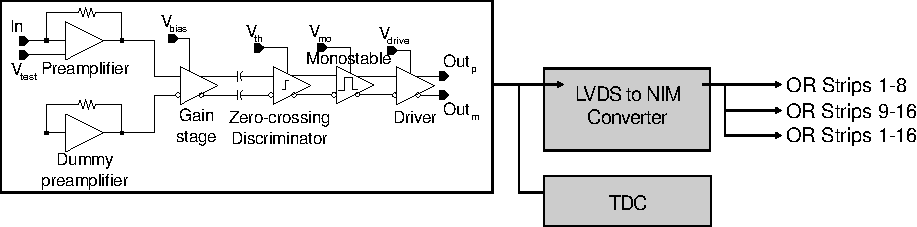
\includegraphics[width = \plotwidth]{fig/chapt5/pulse-processing.pdf}\\
				\caption{\label{fig:DAQ:A}}
			\end{subfigure}
			\begin{subfigure}{\linewidth}
				\centering
				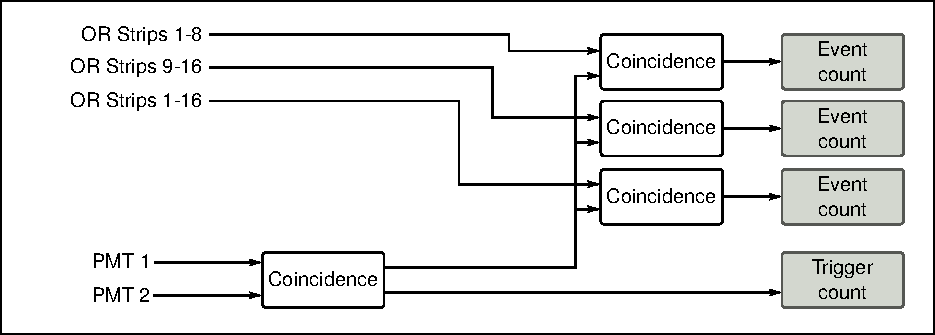
\includegraphics[width = \plotwidth]{fig/chapt5/pulse-processing-2.pdf}
				\caption{\label{fig:DAQ:B}}
			\end{subfigure}
			\caption{\label{fig:DAQ} Signals from the RPC strips are shaped by the FEE described on Figure ~\ref{fig:DAQ:A}. Output LVDS signals are then read-out by a TDC module connected to a computer or converted into NIM and sent to scalers. Figure~\ref{fig:DAQ:B} describes how these converted signals are put in coincidence with the trigger.}
		\end{figure}
		
		\begin{figure}[!h]
			\begin{subfigure}{\linewidth}
				\centering
				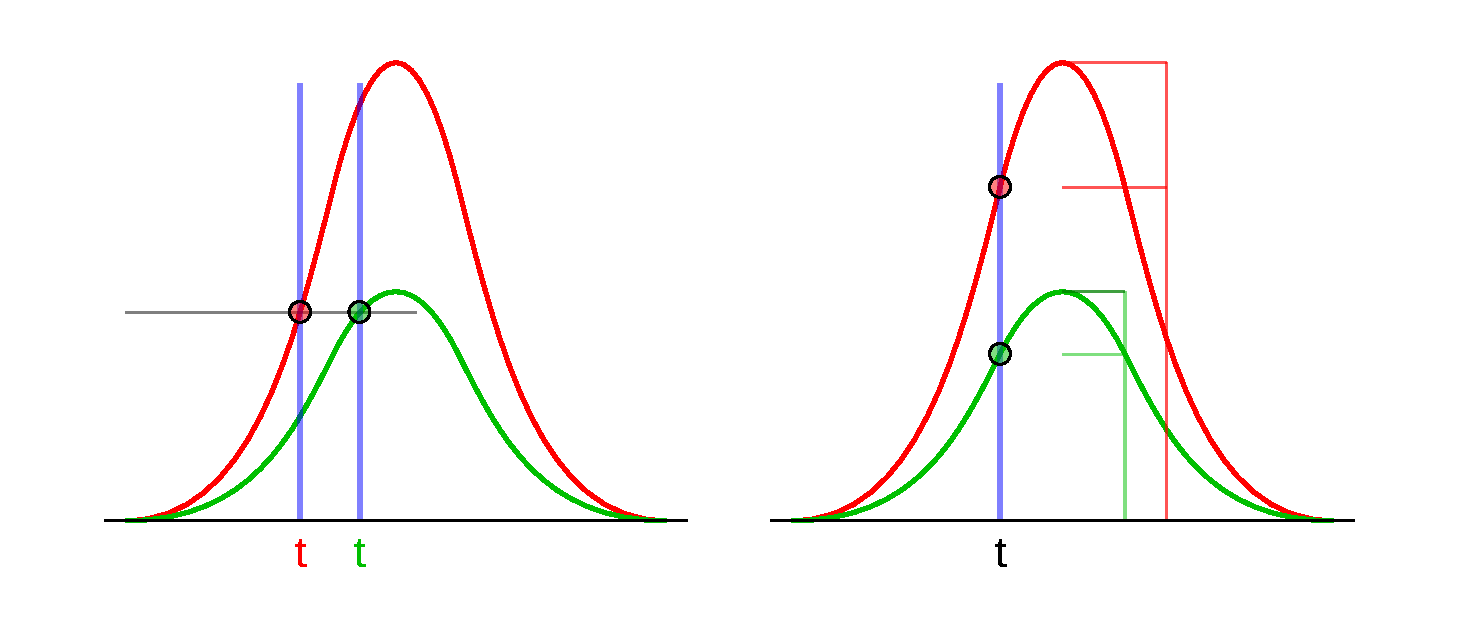
\includegraphics[width = \plotwidth]{fig/chapt5/CFD_1.pdf}\\
				\caption{\label{fig:CFD:A}}
			\end{subfigure}
			\begin{subfigure}{\linewidth}
			    \centering
				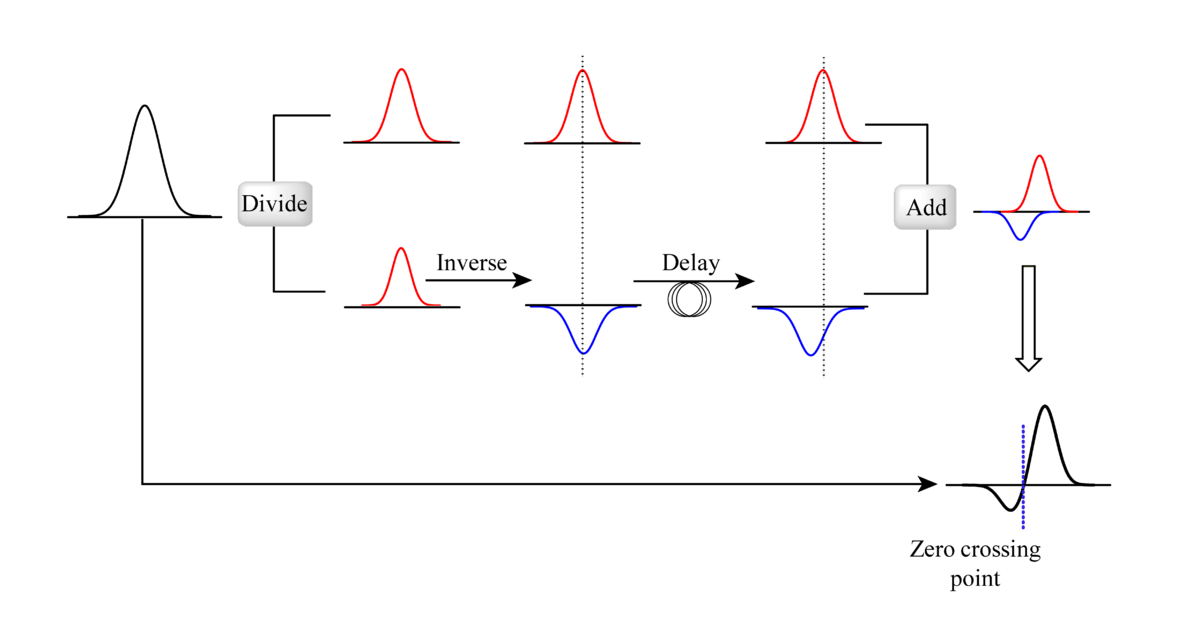
\includegraphics[width = 1.2\plotwidth]{fig/chapt5/CFD_2.png}
				\caption{\label{fig:CFD:B}}
			\end{subfigure}
			\caption{\label{fig:CFD} Description of the principle of a CFD. A comparison of threshold triggering (left) and constant franction triggering (right) is shown in Figure~\ref{fig:CFD:A}. Constant franction triggering is obtained thanks to zero-crossing technique as explained in Figure~\ref{fig:CFD:B}. The signal arriving at the input of the CFD is split into three components. A first one is delayed and connected to the inverting input of a first comparator. A second component is connected to the noninverting input of this first comparator. A third component is connected to the noninverting input of another comparator along with a threshold value connected to the inverting input. Finally, the output of both comparators is fed through an AND gate.}
		\end{figure}

\clearpage{\pagestyle{empty}\cleardoublepage}
